\chapter{Method}
\label{chap:method}
The design of the setup roughly consists of two parts: the nanofabrication of the chip and the experimental setup. We first present a schematic overview of the on-chip design and provide a description of the nanofabrication process. We then describe the experimental setup that includes the external Helmholtz coils and the optical readout.

\section{On-chip design}
\label{sec:on-chip-design}
The design of the chip is based on the proposed on-chip design by \textcite{perdriat}. The design consists of two coplanar loops. In the theory chapter we assumed these loops to be perfectly symmetric and infinitely thin. In reality this is ofcourse not the case and the design needs to be optimized. An important consideration is how the current is distributed in the finite sized tracks and how this affects the magnetic potential. A schematic of the loop design and the distribution of the currents (for $\xi=2$) is shown in \autoref{fig:schematic-tracks}. A finite element simulation in COMSOL is used to model the gradient of the magnetic field. The simulation is done in 3D using a stationary dc-analysis. The curvatures will be presented in \autoref{chap:results}. The thickness of the tracks is \qty{500}{\nano\meter}. Refer to \autoref{tab:sample-dimensions} for a summary of the dimensions of the sample.

\begin{SCfigure}
    \centering
    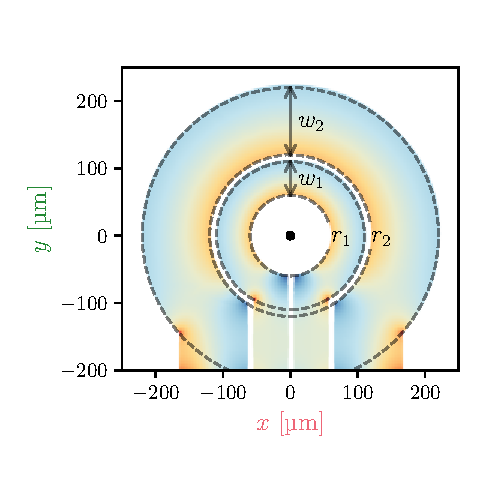
\includegraphics{figures/sample/schematic_tracks.pdf}
    \caption{The design of the on-chip magnetic Paul trap. The dashed lines serve as a guide to the eye. The colormap indicates the current density through the tracks for a current ratio of $\xi = 2$. It can be seen that a majority of the current is concentrated in the inside bends. The extremely high and low currents in the sharp bends are an artefact of the simulation and are not physical. As a reference for the dimensions of the design refer to \autoref{tab:sample-dimensions}.}
    \label{fig:schematic-tracks}
\end{SCfigure}

\begin{SCtable}
    \centering
    \begin{tabular}{lcc}
        \toprule
        \textbf{Parameter} & \textbf{Symbol} & \textbf{Value} \\
        \midrule
        Track thickness & $d$ & \qty{500}{\nm} \\
        Outer track width & $w_1$ & \qty{50}{\um} \\
        Inner track width & $w_2$ & \qty{100}{\um} \\
        Inner loop radius & $r_1$ & \qty{60}{\um} \\
        Outer loop radius & $r_2$ & \qty{120}{\um} \\
        \ce{Si}/Glass hole diameter & & \qty{100}{\um} \\
        \ce{Si}/Glass hole depth & & \qty{15}{\um} \\
        \bottomrule
    \end{tabular}
    \caption{Dimensions of the sample. The radii of the inner and outer loops are their inner radius. Refer to \autoref{fig:schematic-tracks} for further clarification.}
    \label{tab:sample-dimensions}
\end{SCtable}

\subsection{Nanofabrication}
\label{subsec:nanofabrication}
A \qty{9}{\mm} by \qty{5}{\mm} undoped \ce{Si} wafer of \qty{500}{\um} thick is used as a substrate. The substrate is spincoated at \qty{2000}{\rpm} with positive resist AR-P 662.06 and baked at \qty{150}{\celsius} for \qty{3}{\min}. This step is then repeated in order to coat 2 layers in total resulting in a total thickness of \qty{1}{\um}. A lithography step is performed using the Raith 100 EBPG exposing the resist to \qty{400}{\micro\coulomb\per\square\cm}. The resist is developed using a 1:3 mixture of MIBK and isopropanol for \qty{45}{\s}, the development is stopped using isopropanol. The Z-407 sputtering machine deposits a \qty{5}{\nm} \ce{MoSi} sticking layer followed by a \qty{500}{\nm} \ce{Au} layer. The lift-off is performed in acetone and anisole.

Inside of the inner loop of the coil, we mill a hole of roughly \qty{15}{\um} deep with a diameter of \qty{100}{\um} in the \ce{Si} substrate using a \ce{Ga+} focussed ion beam (Aquilos 2 Cryo-FIB). A similar hole is also made in a microscope coverslip. To aid this process a very thin (\qty{5}{\nano\meter}) \ce{Pt} layer is deposited on the glass. Using a micromanipulator a \ce{NdFeB} particle of \qty{12}{\um} is placed inside the \ce{Si} hole. The easiest way to do so is by sticking the particle to the bottom of the needle and then scraping the particle off on the sides of the \ce{Si} hole. The coverslip is placed on top of the \ce{Si} substrate. The holes are carefully aligned by moving the coverslip using a micromanipulator. The coverslip is then glued to the \ce{Si} substrate using an epoxy. The coverslip creates a enclosed environment for the particle to move in. This prevents the particle from escaping the trap. The particle is magnetised by putting the whole sample in a magnetic field of approximately \qty{1.3}{\tesla} for several minutes at room temperature and pressure. \autoref{fig:optical-microscope-image-sample} shows an optical microscope image of the sample.

\begin{figure}
    \centering
    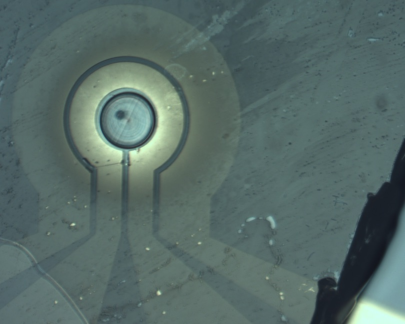
\includegraphics{figures/sample/trap_optical_microscope.pdf}
    \caption{An optical microscope image of the sample. A couple features can be seen in the image 1) in the bottom left is a discoloration due to the epoxy 2) the dark streak in the bottom right is the edge of the cover glass 3) the dark discoloration is the \ce{Pt} layer of the glass. In the center of the trap you can clearly see the \ce{NdFeB} particle. Furthermore, you can see that their is a small misalignment between the hole in the \ce{Si} and hole in the cover glass.}
    \label{fig:optical-microscope-image-sample}
\end{figure}

\section{Experimental setup}
The sample is mounted on a printed circuit board (PCB) with a thick (\qty{1}{\mm}) copper baseplate. The top of the sample is exactly flush with the top of the PCB. Additionally the pads for the wirebonds on the sample and the PCB are aligned and directly next to each other. This allows for very short wirebonds to which significantly reduces the resistance and thus the maximum current that can be applied to the sample. The wirebonds are made of \qty{25}{\um} thick \ce{Al}.

The PCB is then placed inbetween two Helmholtz coils with a diameter of \qty{30}{\mm} and 825 windings. These are the same coils as used in our previous work\cite{eli,mart}. The Helmholtz coils provide the uniform magnetic field to align the sample and the gradient magnetic field to control the vertical position of the particle. A dc current on the order of \qty{0.5}{\ampere} is sent through the coils by two power supplies (Tenma 72-2540).

A microscope objective with a $10\times$ magnification and large working distance is used to provide a visual image of the sample. Additionally a laser (\qty{635}{\nm}, \qty{1}{\milli\watt}) is coupled in. The reflection of the laser is then imaged on a photodiode (ThorLabs PDA36A2). The photodiode is connected to a lock-in amplifier (Zurich Instruments MFLI) allowing for the detection of the motion of the particle. In addition to the photodiode, we can use the camera feed to analyse the motion of the particle.

TODO: schematic of setup

\subsection{Laser analysis}
TODO

\subsection{Camera analysis}
To analyse the camera feed we use a flat-field correction without accounting for the dark frame image. The flat-field is obtained by taking 20 images of the sample when the particle is not trapped and rapdily moving around. The flat-field is then calculated by taking the average of these images. The following transormation is then applied to the frames of the camera feed:
\begin{equation}
    C = \frac{m \cdot R}{F}
    \tag{flat-field correction}
    \label{eq:flat-field-correction}
\end{equation}
where $C$ is the corrected image, $m$ is the average value of the flat-field, $R$ is the raw image and $F$ is the flat-field. The camera feed is processed in grayscale. Due to the flat field correction we get a very clear indication of the position of the particle. This allows us to fit a 2D Gaussian to the particle and determine its position based on the center of the Gaussian.
